\documentclass[12pt, a4paper]{article}
\usepackage[utf8]{inputenc}
\usepackage{tikz}
\usepackage{siunitx}
\usepackage{booktabs}
\usepackage[margin=2cm,footskip=2cm]{geometry}
\usetikzlibrary{automata, positioning, arrows}
\usetikzlibrary{positioning, fit, calc}
\usepackage{tabto}

\begin{document}
\newpage
\section{Solved Problems}
1. Design a two input two output sequence detector which generates an output ‘1’ every time the sequence 1011 is detected. And for all other cases, output ‘0’ is generated. Overlapping sequences are also counted. Draw only the state table and the state diagram.\\
\\
\textbf{\emph{Solution}}:The sequence is 1011. We have to start from $S_{1}$. If we get input 0, then there is no chance to get 1011, so it is confined in $S_{1}$ producing output 0. If we get input 1, then there is a chance to get 1011, and so the control moves to $S_{2}$ producing output 0 (as we have not got 1011 as input still). In $S_{2}$, if we get 0, then there is a chance to get 1011, and so the control moves to $S_{3}$ producing output 0. In $S_{2}$, if we get input 1, then there is a chance to get 1011, considering the last 1. So, the
control will be confined in $S_{2}$, producing output 0.
In $S_{3}$, if we get input 0, then there is no chance to get 1011. In this case, we have to start again
from the beginning, i.e., from $S_{1}$. So, the control moves to $S_{1}$ producing output 0. In the state $S_{3}$, if we get input 0, then there is no chance to get 1011 considering any of the fourth or third and fourth or second, third and fourth or first, second, third, and fourth input combination. In this case, we
have to start again from the beginning, i.e., from $S_{1}$.
So, the control moves to $S_{1}$ producing output 0. If we get input 1, then the string 1011 is achieved, and so the output 1 is
produced. As the overlapping sequence is also accepted, the control moves to $S_{2}$ so that by getting 011, the sequence detector can produce 1. \\
\phantom{20} The state diagram is given. \\
\\
\begin{center}
    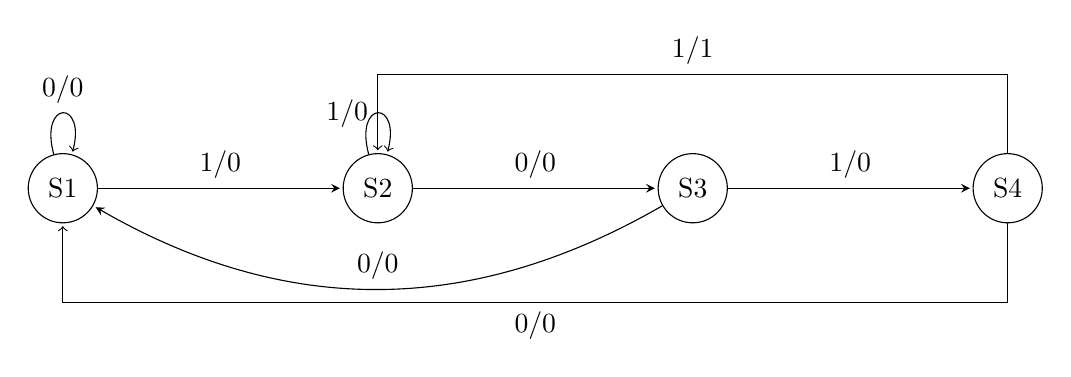
\begin{tikzpicture}[shorten >=1pt,node distance=4cm,on grid,auto]
        \node[state] (q1) {S1};
        \node[state, right of=q1] (q2) {S2};
        \node[state, right of=q2] (q3) {S3};
        \node[state, right of=q3] (q4) {S4};
        \draw[-{stealth[scale=3.0]}]
                (q1) edge[loop above] node{0/0} (q1)
                (q1) edge[above] node{1/0} (q2)
                (q2) edge[loop above, left] node{1/0} (q2)
                (q2) edge[above] node{0/0} (q3)
                (q3) edge[above] node{1/0} (q4)
                (q3) edge[bend left, above] node{0/0} (q1);
        \path[draw,->] 
        (q4.north) -- ++(0, 1cm) -- node [right, above] {1/1}  ++(-8cm,0) -- (q2);
        \path[draw,->] 
        (q4.south) -- ++(0, -1cm) -- node [right, below] {0/0}  ++(-12cm,0) -- (q1);
    \end{tikzpicture}
\end{center}
\phantom{20} The state table for the sequence detector is \\ \\
\begin{center}
    \begin{tabular}{llr}  
    \toprule
    \multicolumn{3}{c}{}{Next State, O/P} \\
    \cmidrule(l){2-3}
    Present State    & X = 0 & = 1 \\
    \midrule
    $S_{1}$      & $S_{1}$, 0    & $S_{2}$, 0      \\
    $S_{2}$      & $S_{3}$, 0    & $S_{4}$, 0      \\
    $S_{3}$      & $S_{1}$, 0    & $S_{2}$, 0      \\
    $S_{4}$      & $S_{1}$, 0    & $S_{2}$, 1      \\
    \bottomrule
    \end{tabular}
\end{center}
\\
2. Design a two input two output sequence detector which generates an output ‘1’ every time the sequence 10101 is detected. And for all other cases, output ‘0’ is generated. Overlapping sequences are also counted. Draw only the state table and the state diagram and make the state assignment.
\newpage
\textbf{\emph{Solution}}: 
\begin{center}
    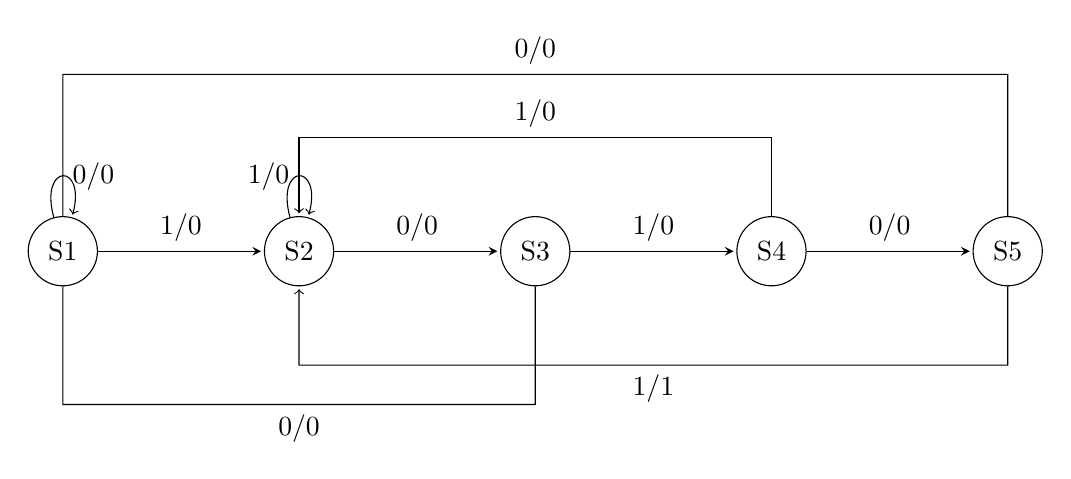
\begin{tikzpicture}[shorten >=1pt,node distance=3cm,on grid,auto]
        \node[state] (q1) {S1};
        \node[state, right of=q1] (q2) {S2};
        \node[state, right of=q2] (q3) {S3};
        \node[state, right of=q3] (q4) {S4};
        \node[state, right of=q4] (q5) {S5};
        \draw[-{stealth[scale=3.0]}]
                (q1) edge[loop above, right] node{0/0} (q1)
                (q1) edge[above] node{1/0} (q2)
                (q2) edge[loop above, left] node{1/0} (q2)
                (q2) edge[above] node{0/0} (q3)
                (q3) edge[above] node{1/0} (q4)
                (q4) edge[above] node{0/0} (q5);
        \path[draw,->] 
        (q4.north) -- ++(0, 1cm) -- node [right, above] {1/0}  ++(-6cm,0) -- (q2);
        \path[draw,->] 
        (q3.south) -- ++(0, -1.5cm) -- node [right, below] {0/0}  ++(-6cm,0) -- (q1)
        (q5.north) -- ++(0, 1.8cm) -- node [left, above] {0/0}  ++(-12cm,0) -- (q1)
        (q5.south) -- ++(0, -1cm) -- node [left, below] {1/1}  ++(-9cm,0) -- (q2);
    \end{tikzpicture}
\end{center}
\phantom{20}\hspace{2ex} The state diagram is constructed previously. \\
\phantom{20}\hspace{2ex} Here, the overlapping sequence is 101.
\begin{center}
    \begin{tikzpicture}
        % \draw[draw=black] rectangle ++(2, 0.4) node[pos=.5] {1 0 1 0 1};
        % \draw[draw=black, width = 0.5\textwidth] rectangle ++(1, 0.6) node[pos=.5];
        \node (inner1) [draw] {1 0 1 0 1};
        % \node (outer) [fit=(inner1)] {};
        \coordinate (o) at ($(inner2.north)!1/3!(inner2.south)$);
        \draw [black, densely dashed] (outer.north west) rectangle (outer.south east |- o) node [below=5mm of inner1] {};
    \end{tikzpicture}
\end{center}
The state table for the sequence detector is \\ \\
\begin{center}
    \begin{tabular}{llr}  
    \toprule
    \multicolumn{3}{c}{}{Next State, O/P} \\
    \cmidrule(l){2-3}
    Present State    & X = 0 & = 1 \\
    \midrule
    \phantom{20}\hspace{2ex}$S_{1}$      & $S_{1}$, 0    & $S_{2}$, 0      \\
    \phantom{20}\hspace{2ex}$S_{2}$      & $S_{3}$, 0    & $S_{4}$, 0      \\
    \phantom{20}\hspace{2ex}$S_{3}$      & $S_{1}$, 0    & $S_{2}$, 0      \\
    \phantom{20}\hspace{2ex}$S_{4}$      & $S_{1}$, 0    & $S_{2}$, 0      \\
    \phantom{20}\hspace{2ex}$S_{5}$      & $S_{1}$, 0    & $S_{2}$, 1      \\
    \bottomrule
    \end{tabular}
\end{center}
\phantom{20} For doing the state assignment, we have to assign the states to some binary numbers. Here are five states, so we have to take a binary string of length three because $2^3 = 8 > 5$. \\
\phantom{20} Let us assign 000 as $S_{1}$, 001 as $S_{2}$, 011 as $S_{3}$, 010 as $S_{4}$, and 100 as $S_{5}$. \\
\phantom{20} After doing the state assignment, the state table becomes \\ \\
\begin{center}
    \begin{tabular}{lrrrr}  
    \toprule
    \multicolumn{5}{c} {Present State}{}{Next State ($Y_{1}$,$Y_{2}$)} {O/P (z)}\\
    \cmidrule(lr){2-3} 
    \cmidrule(lr){4-5} 
    ($y_{2}$,$y_{1}$) & X = 0 & = 1 & = 0 & = 1 \\
    \midrule
    \phantom{20}000 & \phantom{20}000 & 001 & 0 & 0      \\
    \phantom{20}011 & \phantom{20}011 & 001 & 0 & 0      \\
    \phantom{20}011 & \phantom{20}010 & 000 & 0 & 0      \\
    \phantom{20}010 & \phantom{20}100 & 001 & 0 & 0      \\
    \phantom{20}100 & \phantom{20}000 & 001 & 0 & 1      \\
    \bottomrule
    \end{tabular}
\end{center}
\newpage
3. Find the equivalent partition for the following machine. \\ \\
\begin{center}
    \begin{tabular}{llr}  
    \toprule
    \multicolumn{3}{c}{}{Next State, z} \\
    \cmidrule(l){2-3}
    Present State    & X = 0 & X = 1 \\
    \midrule
    \phantom{20}\hspace{2ex}A      & B, 0    & C, 1      \\
    \phantom{20}\hspace{2ex}B      & A, 0    & E, 1      \\
    \phantom{20}\hspace{2ex}C      & D, 1    & E, 1      \\
    \phantom{20}\hspace{2ex}D      & E, 1    & B, 1      \\
    \phantom{20}\hspace{2ex}E      & C, 1    & B, 1      \\
    \bottomrule
    \end{tabular}
\end{center}
\textbf{\emph{Solution}}: For a string length 0 (i.e., for no input), there is no output. So, all the states are equivalent.
It is called 0-equivalent. We can write \[P_{0} = (ABCDE)\] \\
\phantom{20} For string length 1, there are two types of inputs—0 and 1. The states A and B give output 0 for input 0 and states C, D, and E give output 1 for input 0. All of the states give output 1 for input 1. \\
\phantom{20} So, the states in the set $P_{0}$ are divided into (AB) and (C, D, E). We can write \[P_{1} = ((AB)(CDE))\] \\
\phantom{20} Here A and E are 1-distinguishable because they produce different outputs for input string length 1. \\
\phantom{20} For input string length 2, check the distinguishability by the next state combination. \\
\phantom{20} The states A and B for input 0 produce next states B and A, respectively, and produce next \\ 
states C and E for input 1. B and A belong to same set, and C and E also belong to the same set. \\
So, AB cannot be partitioned for the input string length 2. \\
\phantom{20} The states CDE for input 0 produce next states D, E, D, respectively, and produce next states E, B, B for input 1. D, E belong to same set but B and E belong to different sets. So, the set (CDE) is portioned into (C) and (DE). The new partition becomes \[P_{2} = (A)(B)(C)(DE)\] \\
\phantom{20} Next, we have to check for input string length 4. Three subsets contain single state—A, B, and C, and cannot be partitioned further. \\
\phantom{20}  The states D and E produce the next states E and D, respectively, for input 0 and the next state B for each of the states for input 1. D and E belong to same set, and so D and E cannot be partitioned further. The partition is the same as P3. So, the partition P3 is the equivalent partition of the machine. \\ \\
\textbf{\emph{Minimization}}: We know that the equivalent partition is unique. So, P3 = (A)(B)(C)(DE) is the unique combination. Here, every single set represents one state of the minimized machine.
\newpage
Let us rename these partitions for simplification. \\
\phantom{20}Rename (A) as S1 , (B) as S2, (C) as S3, and (DE) as S4. \\
\phantom{20}The minimized machine becomes \\ \\
\begin{center}
    \begin{tabular}{llr}  
    \toprule
    \multicolumn{3}{c}{}{Next State, z} \\
    \cmidrule(l){2-3}
    Present State    & X = 0 & X = 1 \\
    \midrule
    \phantom{20}$S_{1}$(A)      & $S_{2}$, 0    & $S_{3}$, 1      \\
    \phantom{20}$S_{2}$(B)      & $S_{1}$, 0    & $S_{4}$, 1      \\
    \phantom{20}$S_{3}$(C)      & $S_{4}$, 1    & $S_{4}$, 1      \\
    \phantom{20}$S_{1}$(DE)     & $S_{4}$, 1    & $S_{2}$, 1      \\
    \bottomrule
    \end{tabular}
\end{center}
4. Find the equivalent partition of the following machine. \\
\begin{center}
    \begin{tabular}{llr}  
    \toprule
    \multicolumn{3}{c}{}{Next State, z} \\
    \cmidrule(l){2-3}
    Present State    & X = 0 & X = 1 \\
    \midrule
    \phantom{20}\hspace{2ex}A      & B, 0    & D, 1      \\
    \phantom{20}\hspace{2ex}B      & D, 1    & F, 1      \\
    \phantom{20}\hspace{2ex}C      & F, 1    & B, 1      \\
    \phantom{20}\hspace{2ex}D      & F, 0    & A, 1      \\
    \phantom{20}\hspace{2ex}E      & C, 0    & A, 1      \\
    \phantom{20}\hspace{2ex}F      & C, 1    & B, 1      \\
    \bottomrule
    \end{tabular}
\end{center}
\textbf{\emph{Solution}}: The partitions are \\
\phantom{20}\hspace{5ex} P0 = (ABCDEF) \\
\phantom{20}\hspace{5ex} P1 = (ADE)(BCF) (Depending on o/p for i/p 0) \\
\phantom{20}\hspace{5ex} P2 = (ADE)(B)(CF) (For i/p 0, the next state of B goes to another set) \\
\phantom{20}\hspace{5ex} P3 = (A)(DE)(B)(CF) (For i/p 0, the next state of A goes to another set) \\
\phantom{20}\hspace{5ex} P4 = (A)(DE)(B)(CF) \\
As $P_{3}$ and $P_{4}$ are the same, $P_{3}$ is the equivalent partition. \\
\textbf{\emph{Minimization}}: We know that the equivalent partition is unique. So, P4 = (A)(DE)(B)(CF) is the
unique combination. Here, every single set represents one state of the minimized machine. \\
\phantom{20} Let us rename these partitions for simplification. \\
\phantom{20} Rename (A) as $S_{1}$, (B) as $S_{2}$, (DE) as $S_{3}$, and (CF) as $S_{4}$. \\
\phantom{20} The minimized machine becomes \\ \\
\begin{center}
    \begin{tabular}{llr}  
    \toprule
    \multicolumn{3}{c}{}{Next State, z} \\
    \cmidrule(l){2-3}
    Present State    & X = 0 & = 1 \\
    \midrule
    \phantom{20}\hspace{2ex}$S_{1}$(A)      & B, 0    & D, 1      \\
    \phantom{20}\hspace{2ex}$S_{2}$(B)      & D, 1    & F, 1      \\
    \phantom{20}\hspace{2ex}$S_{3}$(DE)      & F, 1    & B, 1      \\
    \phantom{20}\hspace{2ex}$S_{4}$(CF)      & F, 0    & A, 1      \\
    \bottomrule
    \end{tabular}
\end{center}
\end{document}
